\documentclass[a4j,twoside,openright,11pt]{jarticle}
%
\usepackage{amsmath,amssymb}
\usepackage{bm}
\usepackage{graphicx}
\usepackage{ascmac}
\usepackage{listliketab}
\usepackage{url}
\usepackage{listings}

\setlength{\textwidth}{15.92cm}
\setlength{\oddsidemargin}{0mm}
\setlength{\evensidemargin}{0mm}
\setlength{\topmargin}{-1cm}
\setlength{\textheight}{23.5cm}
\setlength{\footskip}{18mm}

%
\pagestyle{plain}

\begin{document}
\begin{screen}
\huge
\begin{center}
{\bf 機械工学実験2\\サイホン管の流れと流体抵抗の測定}\\
\end{center}

\normalsize
\begin{flushright}
九州工業大学 機械知能工学科 機械知能コース  坂本 悠作\\学籍番号:13104069 \hspace{0.2in}実験日 2015年5月8日  提出日 2015年5月20日
\end{flushright}
\end{screen}


\section{実験目的}
サイホン管を流れる水量と菅入口の出口間の落差を測定し、サイホンヘッドと管内流速との関係をベルヌーイの式で得られる結果を比較し、流体のエネルギー保存則について学ぶ。
\section{実験方法}
\subsection{実験手順}
\begin{enumerate}
\item ボール弁を全開にして、サイホン管路を水槽の水で満たす。
\item 実験条件として、大気圧、乾湿球温度計、水温を調べる。
\item 実験開始時点の水深を1350mmに設定し、各計測器(差圧系、電磁流量計)の値を読み取る
\item ボール弁を全開にしてサイホン流れを開始する
\item 設定落差に至った時点で、合図し、データを一斉に読み取る
\item 落差の設定点数に合わせて手順5を繰り返す
\item ボール弁の損失を測定する。開度は25㎜毎に次の値に設定する
\begin{itemize}
\item 弁の開度:7/8
\item 弁の開度:3/4
\item 弁の開度:1/2
\end{itemize}
\item ボール弁を全閉にして、実験終了時点の水深、測定値の値を読みとる
\item 記録の確認・点検後実験を終了する。
\end{enumerate}
\subsection{記号・計算式のまとめ}
\begin{itemize}
\item d=50[mm]
\item 水槽の水深Y[mm]
\item 電磁流量計の指示値Q[$m^3/s$]
\item 圧力センサーの指示値R[kPa]
\item 差圧計の指示値S[kPa]
\item 経過時間T[s]
\item 重力加速度g=9.80665[$m/s^2$]
\item 水槽幅:2.0[m]
\item 水槽奥行き:1.0[m]
\item 水槽高さ:1.4[m]
\item サイホン管の出口部の位置$Y_0$=-130[mm]
\item サイホンヘッドH[m]\\
\begin{equation}
H[m]=(Y-Y_0)/1000[m]
\end{equation}
\item 管内流速V[m/s]
\item ブラジウスの式(適用範囲$3 \times 10^3 \leq R_e \leq10^5$)\\
\item 管内圧力
\begin{equation}
\lambda=0.3164 \times R_e^{-0.25}
\end{equation}
\item 流量係数(エルボ):$\alpha_b$
\end{itemize}
\begin{equation}
\alpha_b=\frac{V}{ \sqrt{2 \Delta P_b / \rho }}
\end{equation}
\section{実験結果}
\subsection{測定結果}
\newpage
\subsection{測定結果のまとめ}

\begin{figure}[htbp]
\begin{center}
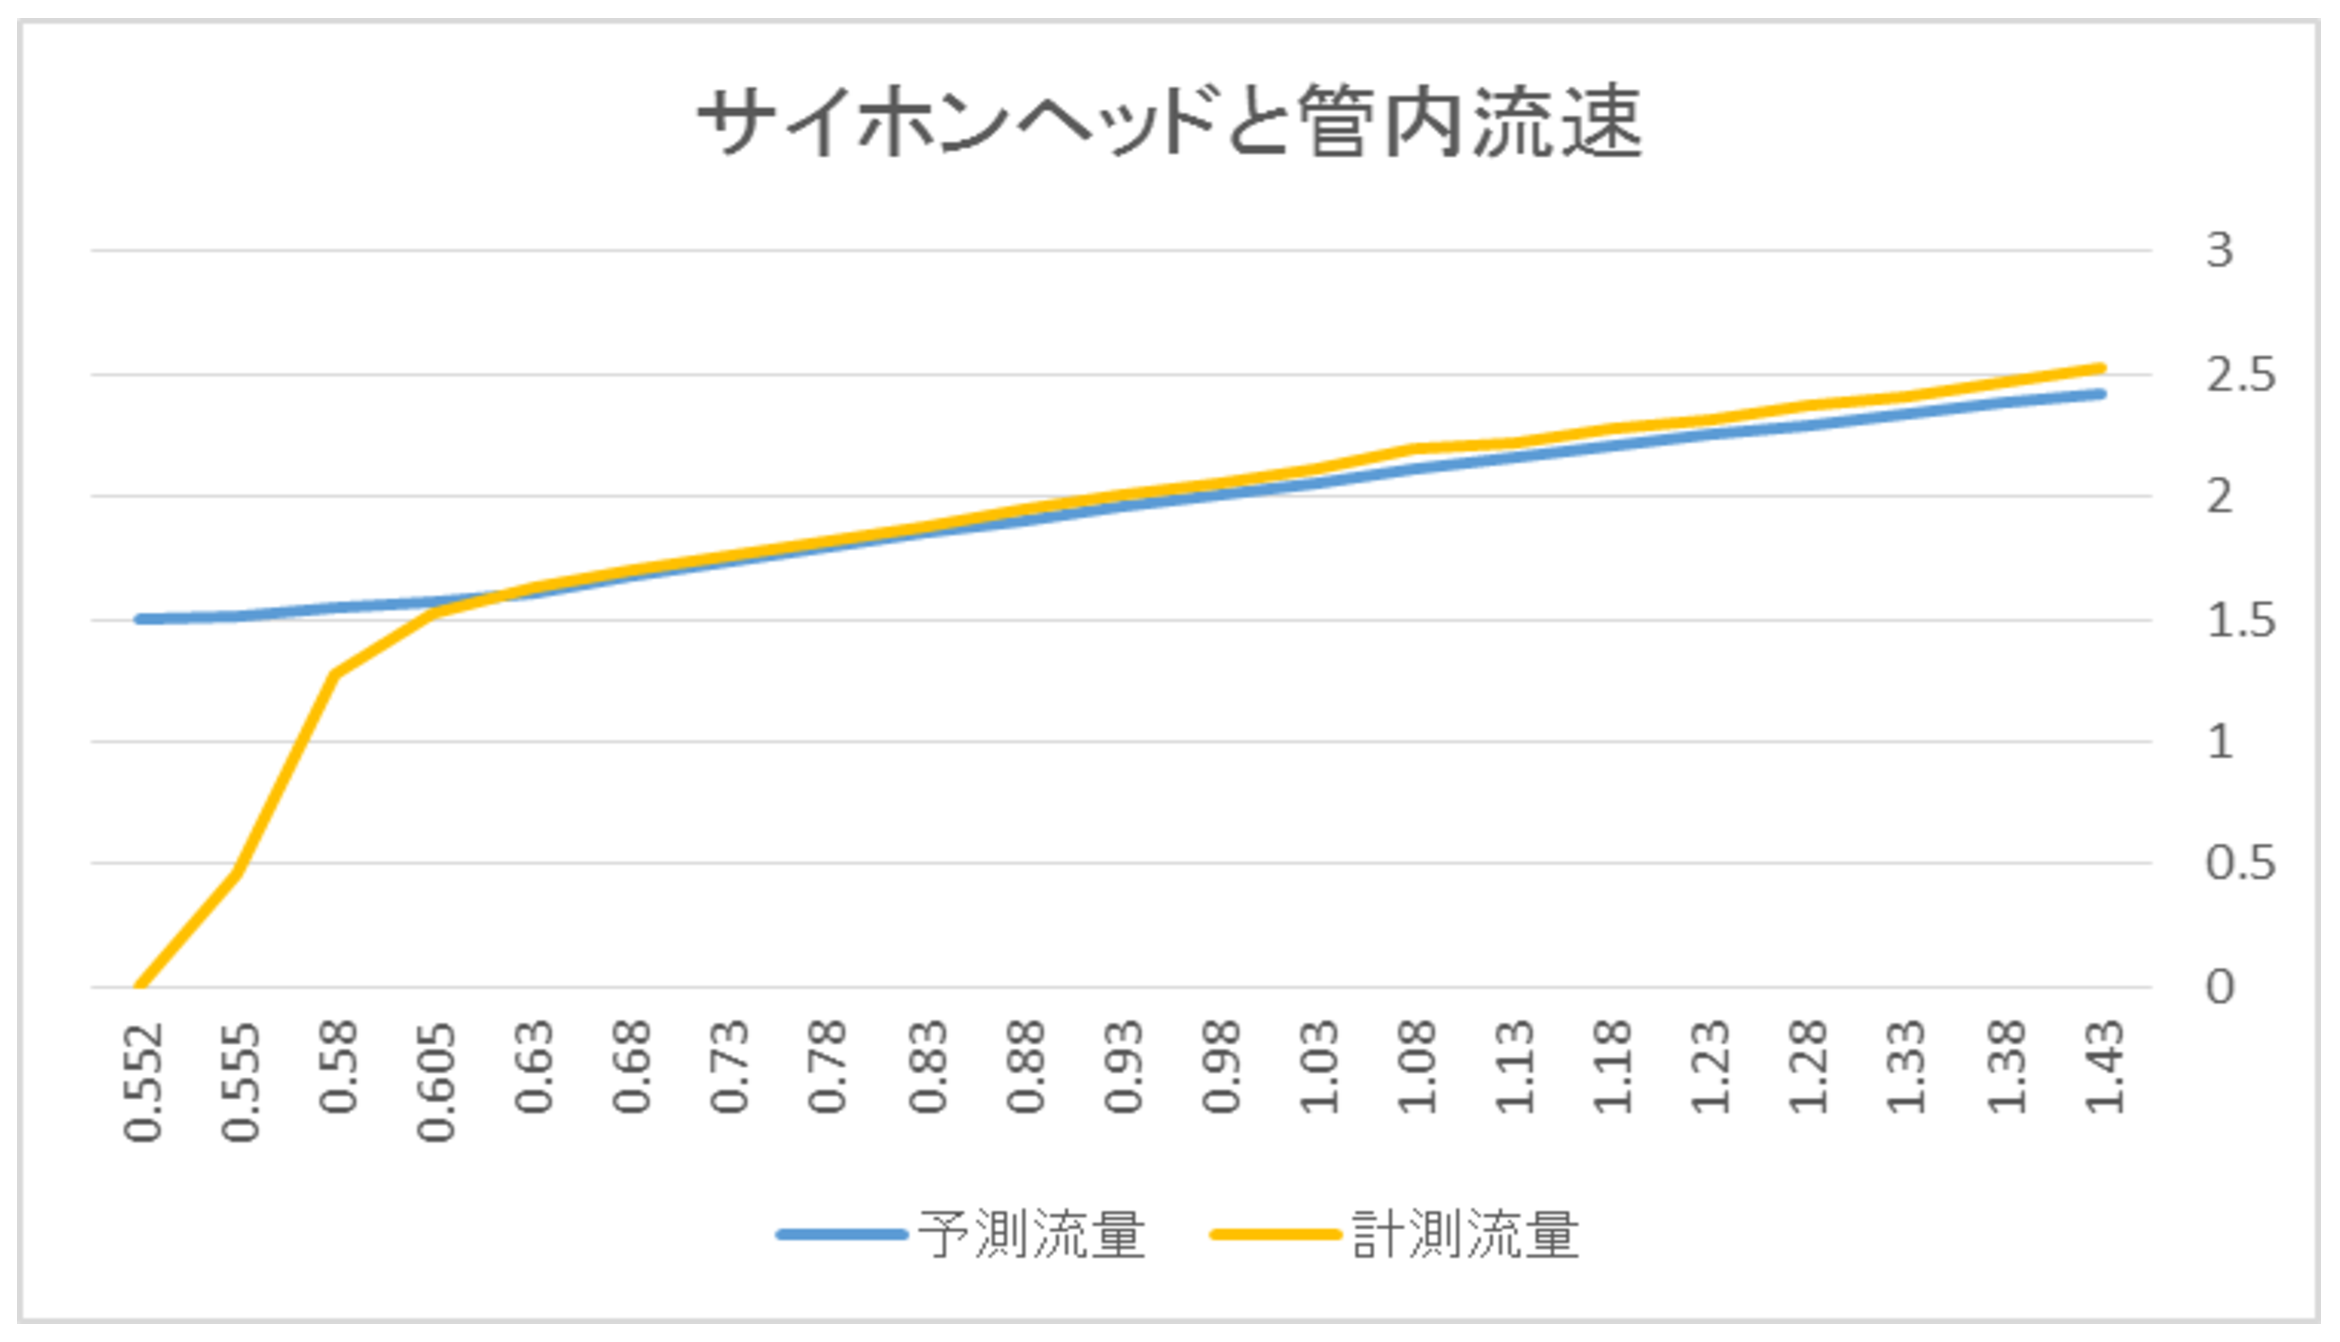
\includegraphics[width=12cm]{4.eps}
\end{center}
\caption{サイホンヘッドと管内流速(横軸:サイホンヘッドH 縦軸:管内流速)}
\end{figure}

\begin{figure}[htbp]
\begin{center}
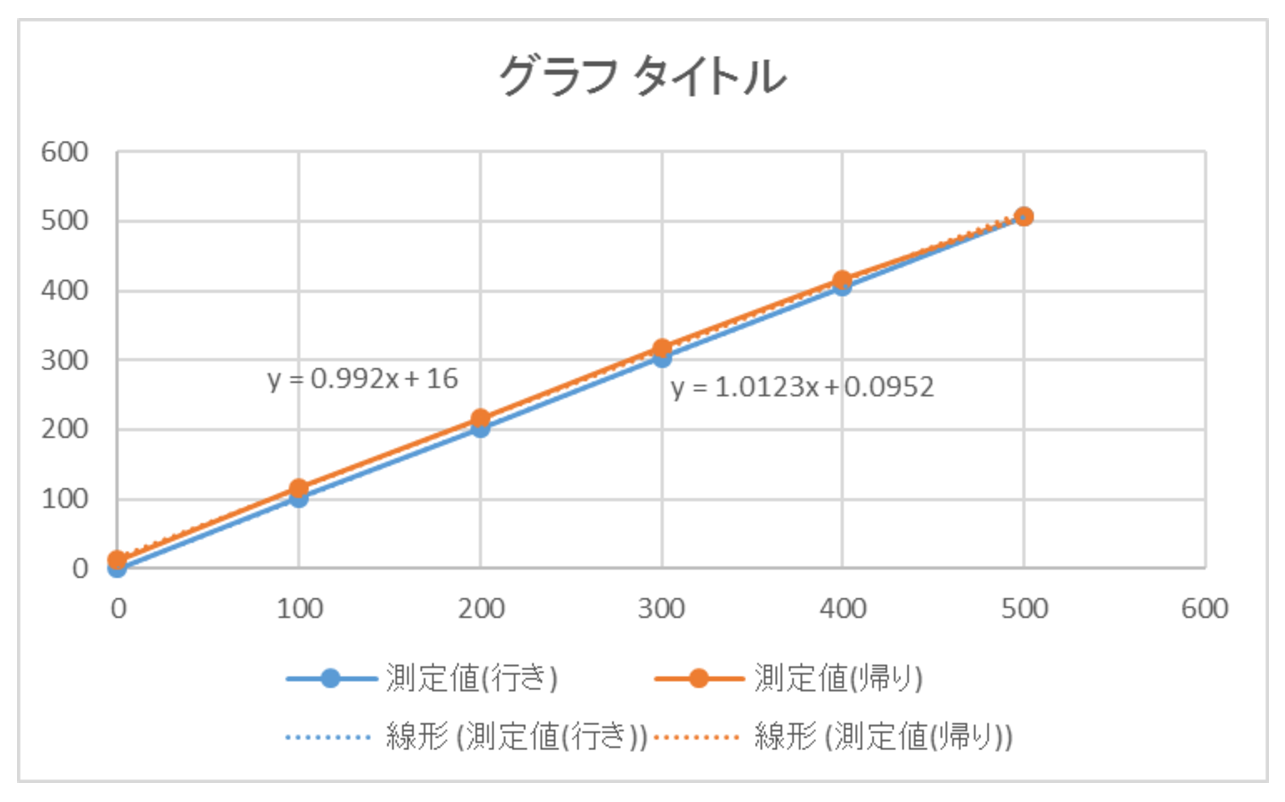
\includegraphics[width=12cm]{1.eps}
\end{center}
\caption{サイホンヘッドと無次元管内圧(横軸:サイホンヘッドH 縦軸:無次元管内圧力)}
\end{figure}

\begin{figure}[htbp]
\begin{center}
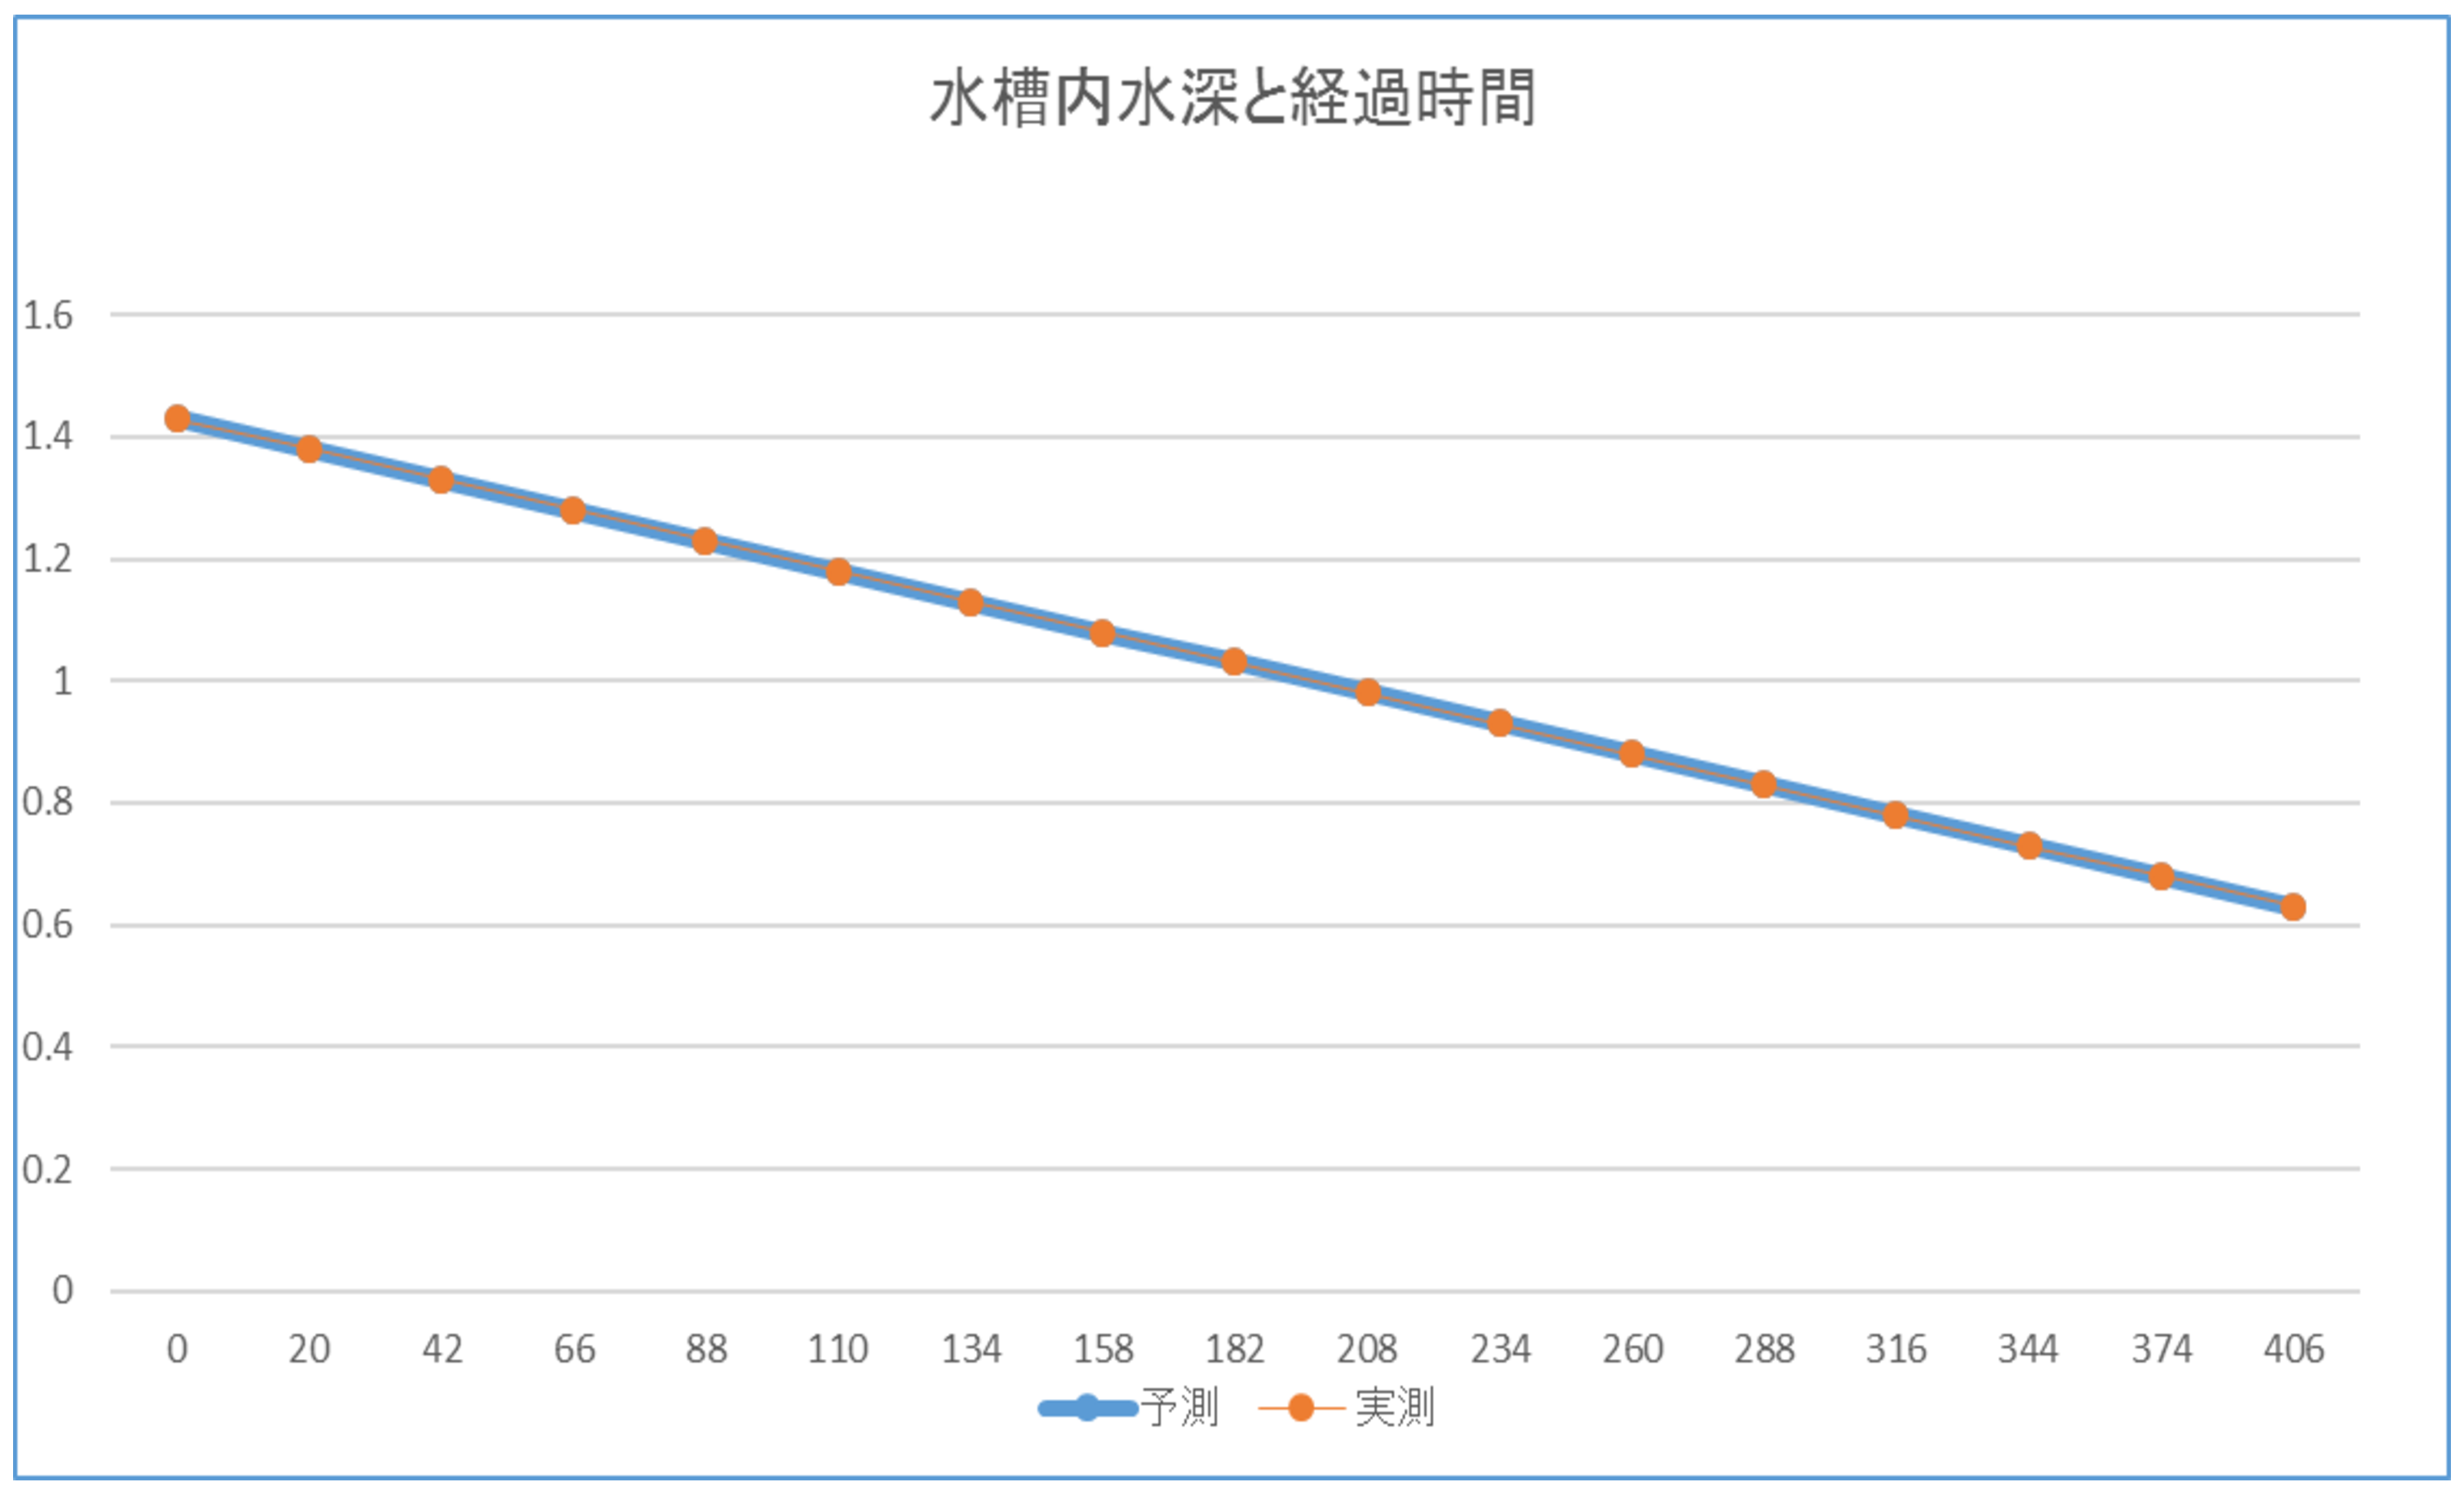
\includegraphics[width=12cm]{2.eps}
\end{center}
\caption{水槽内水深と経過時間(横軸:時間 縦軸:水槽水深)}
\end{figure}

\begin{figure}[htbp]
\begin{center}
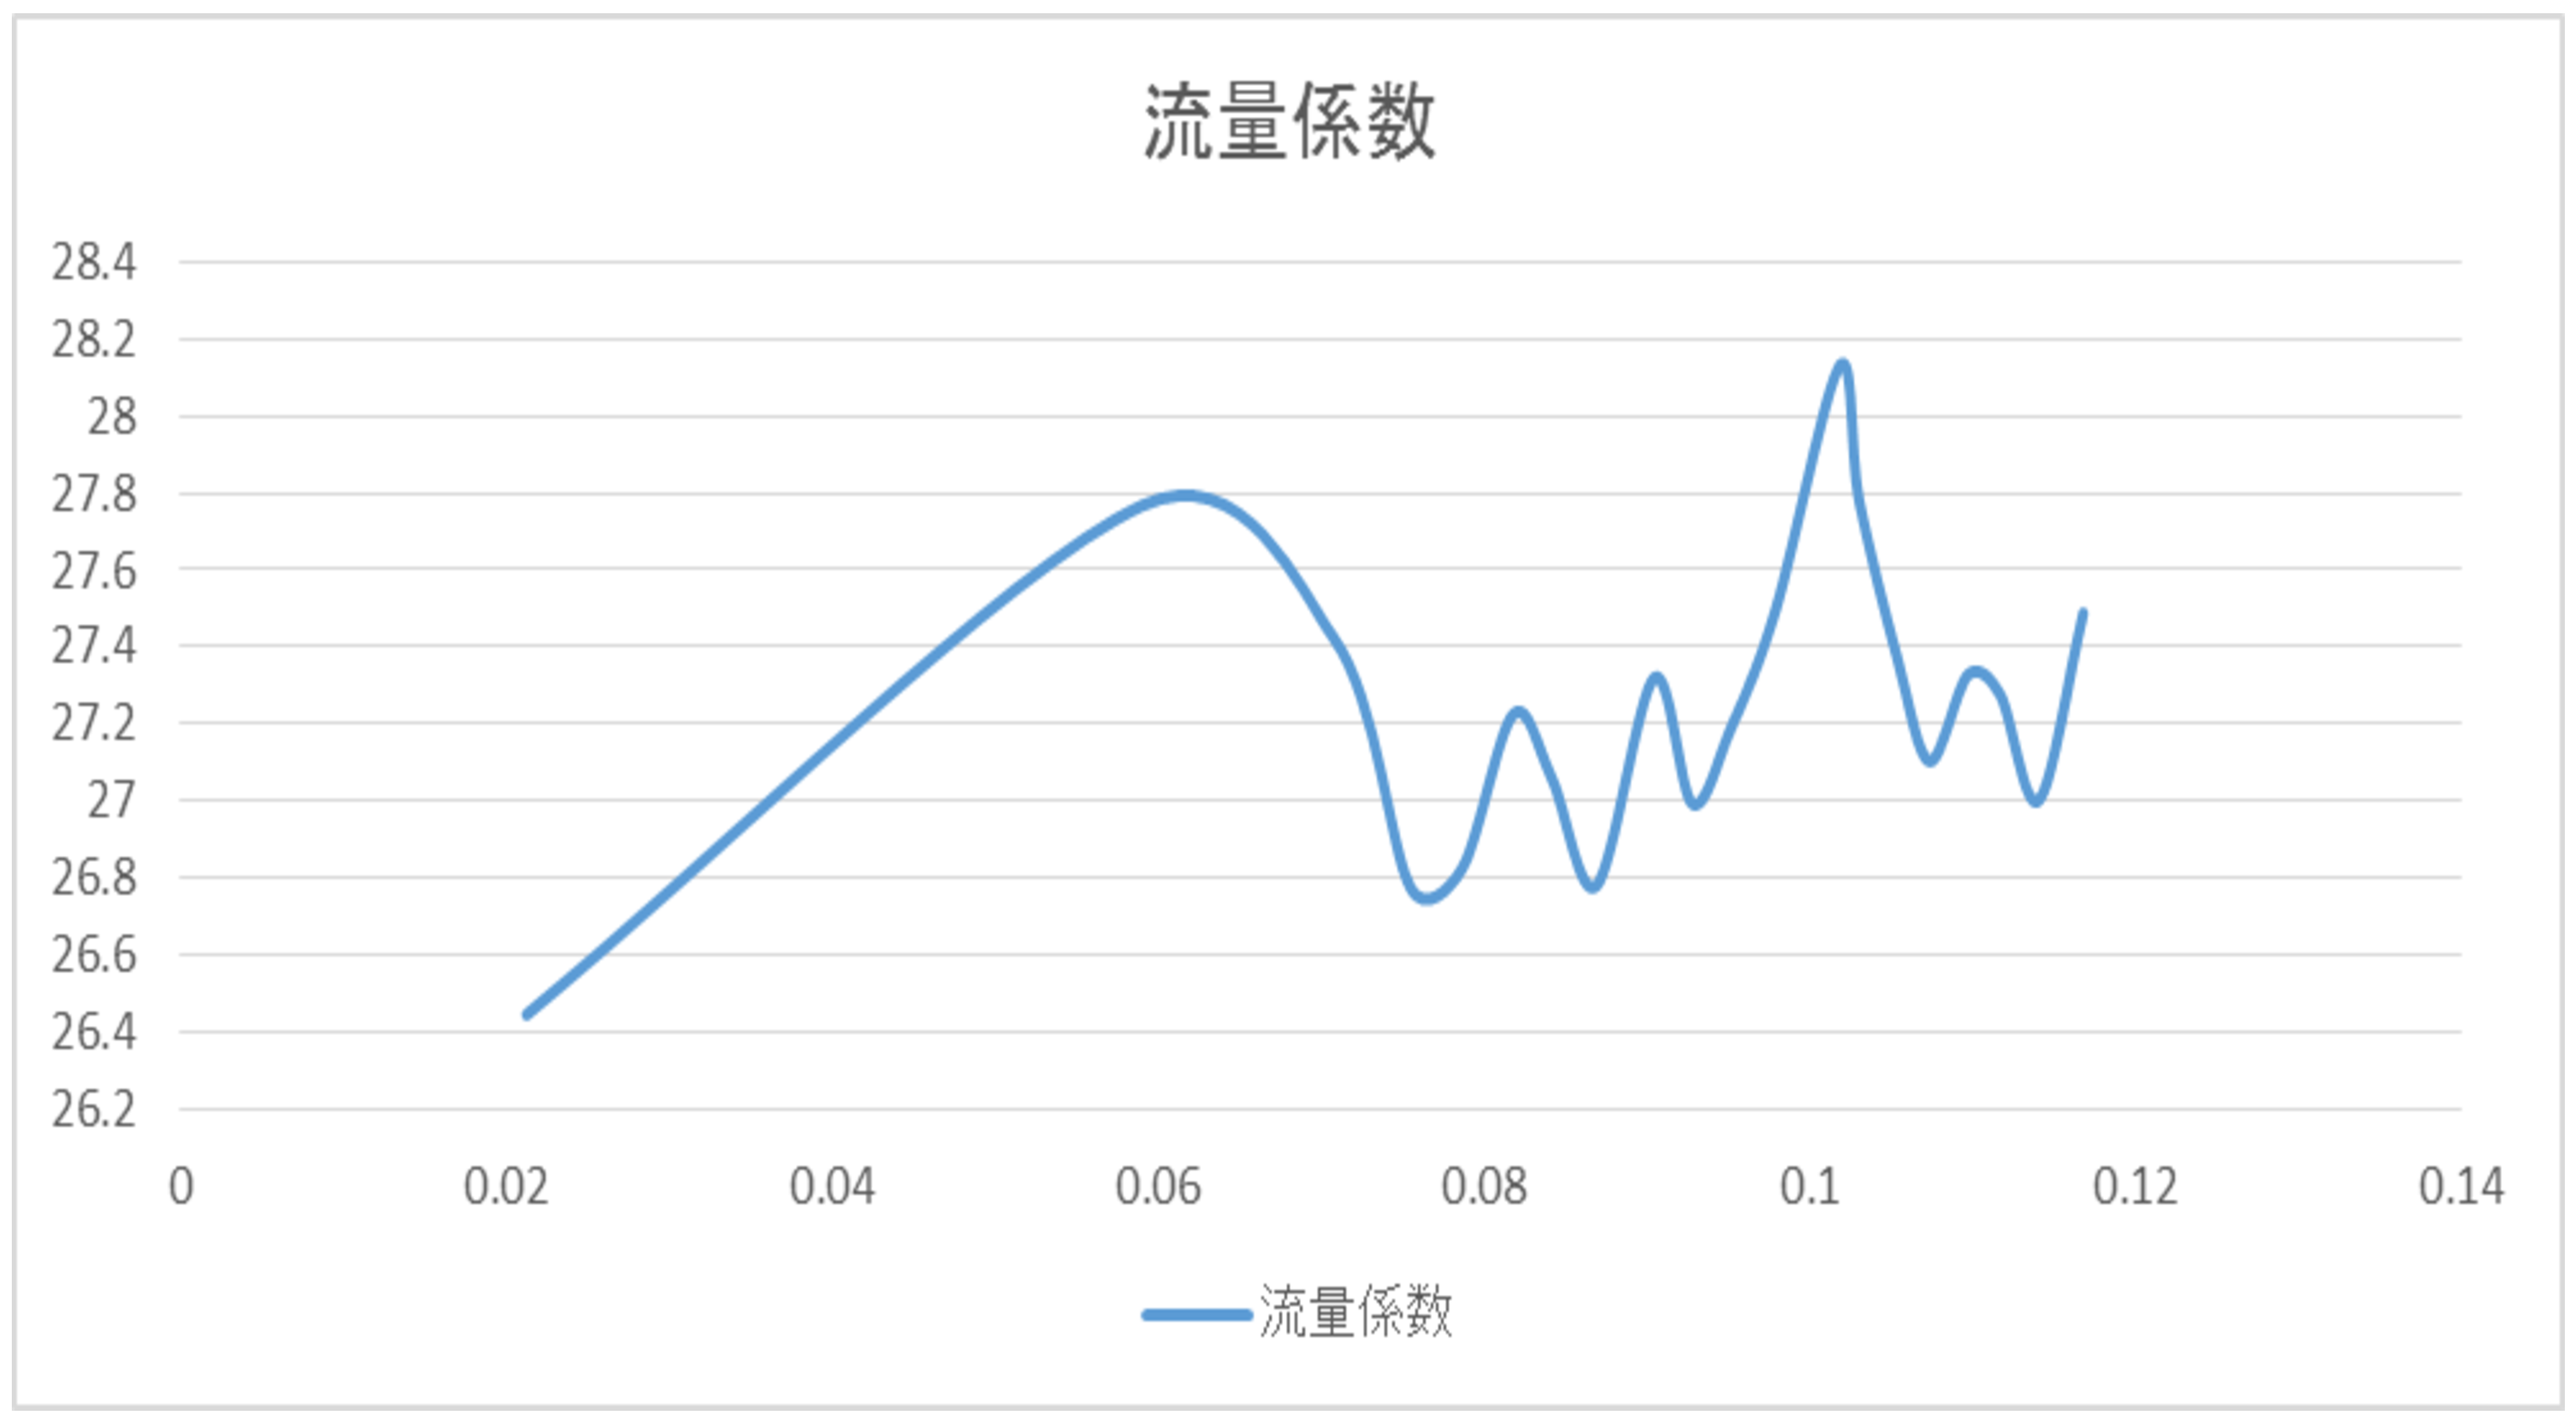
\includegraphics[width=12cm]{3.eps}
\end{center}
\caption{管レイノルズ数とエルボ流量計数の関係(横軸:管レイノルズ数($\times10^6$)  縦軸:エルボ流量計数)}
\end{figure}

\begin{figure}[htbp]
\begin{center}
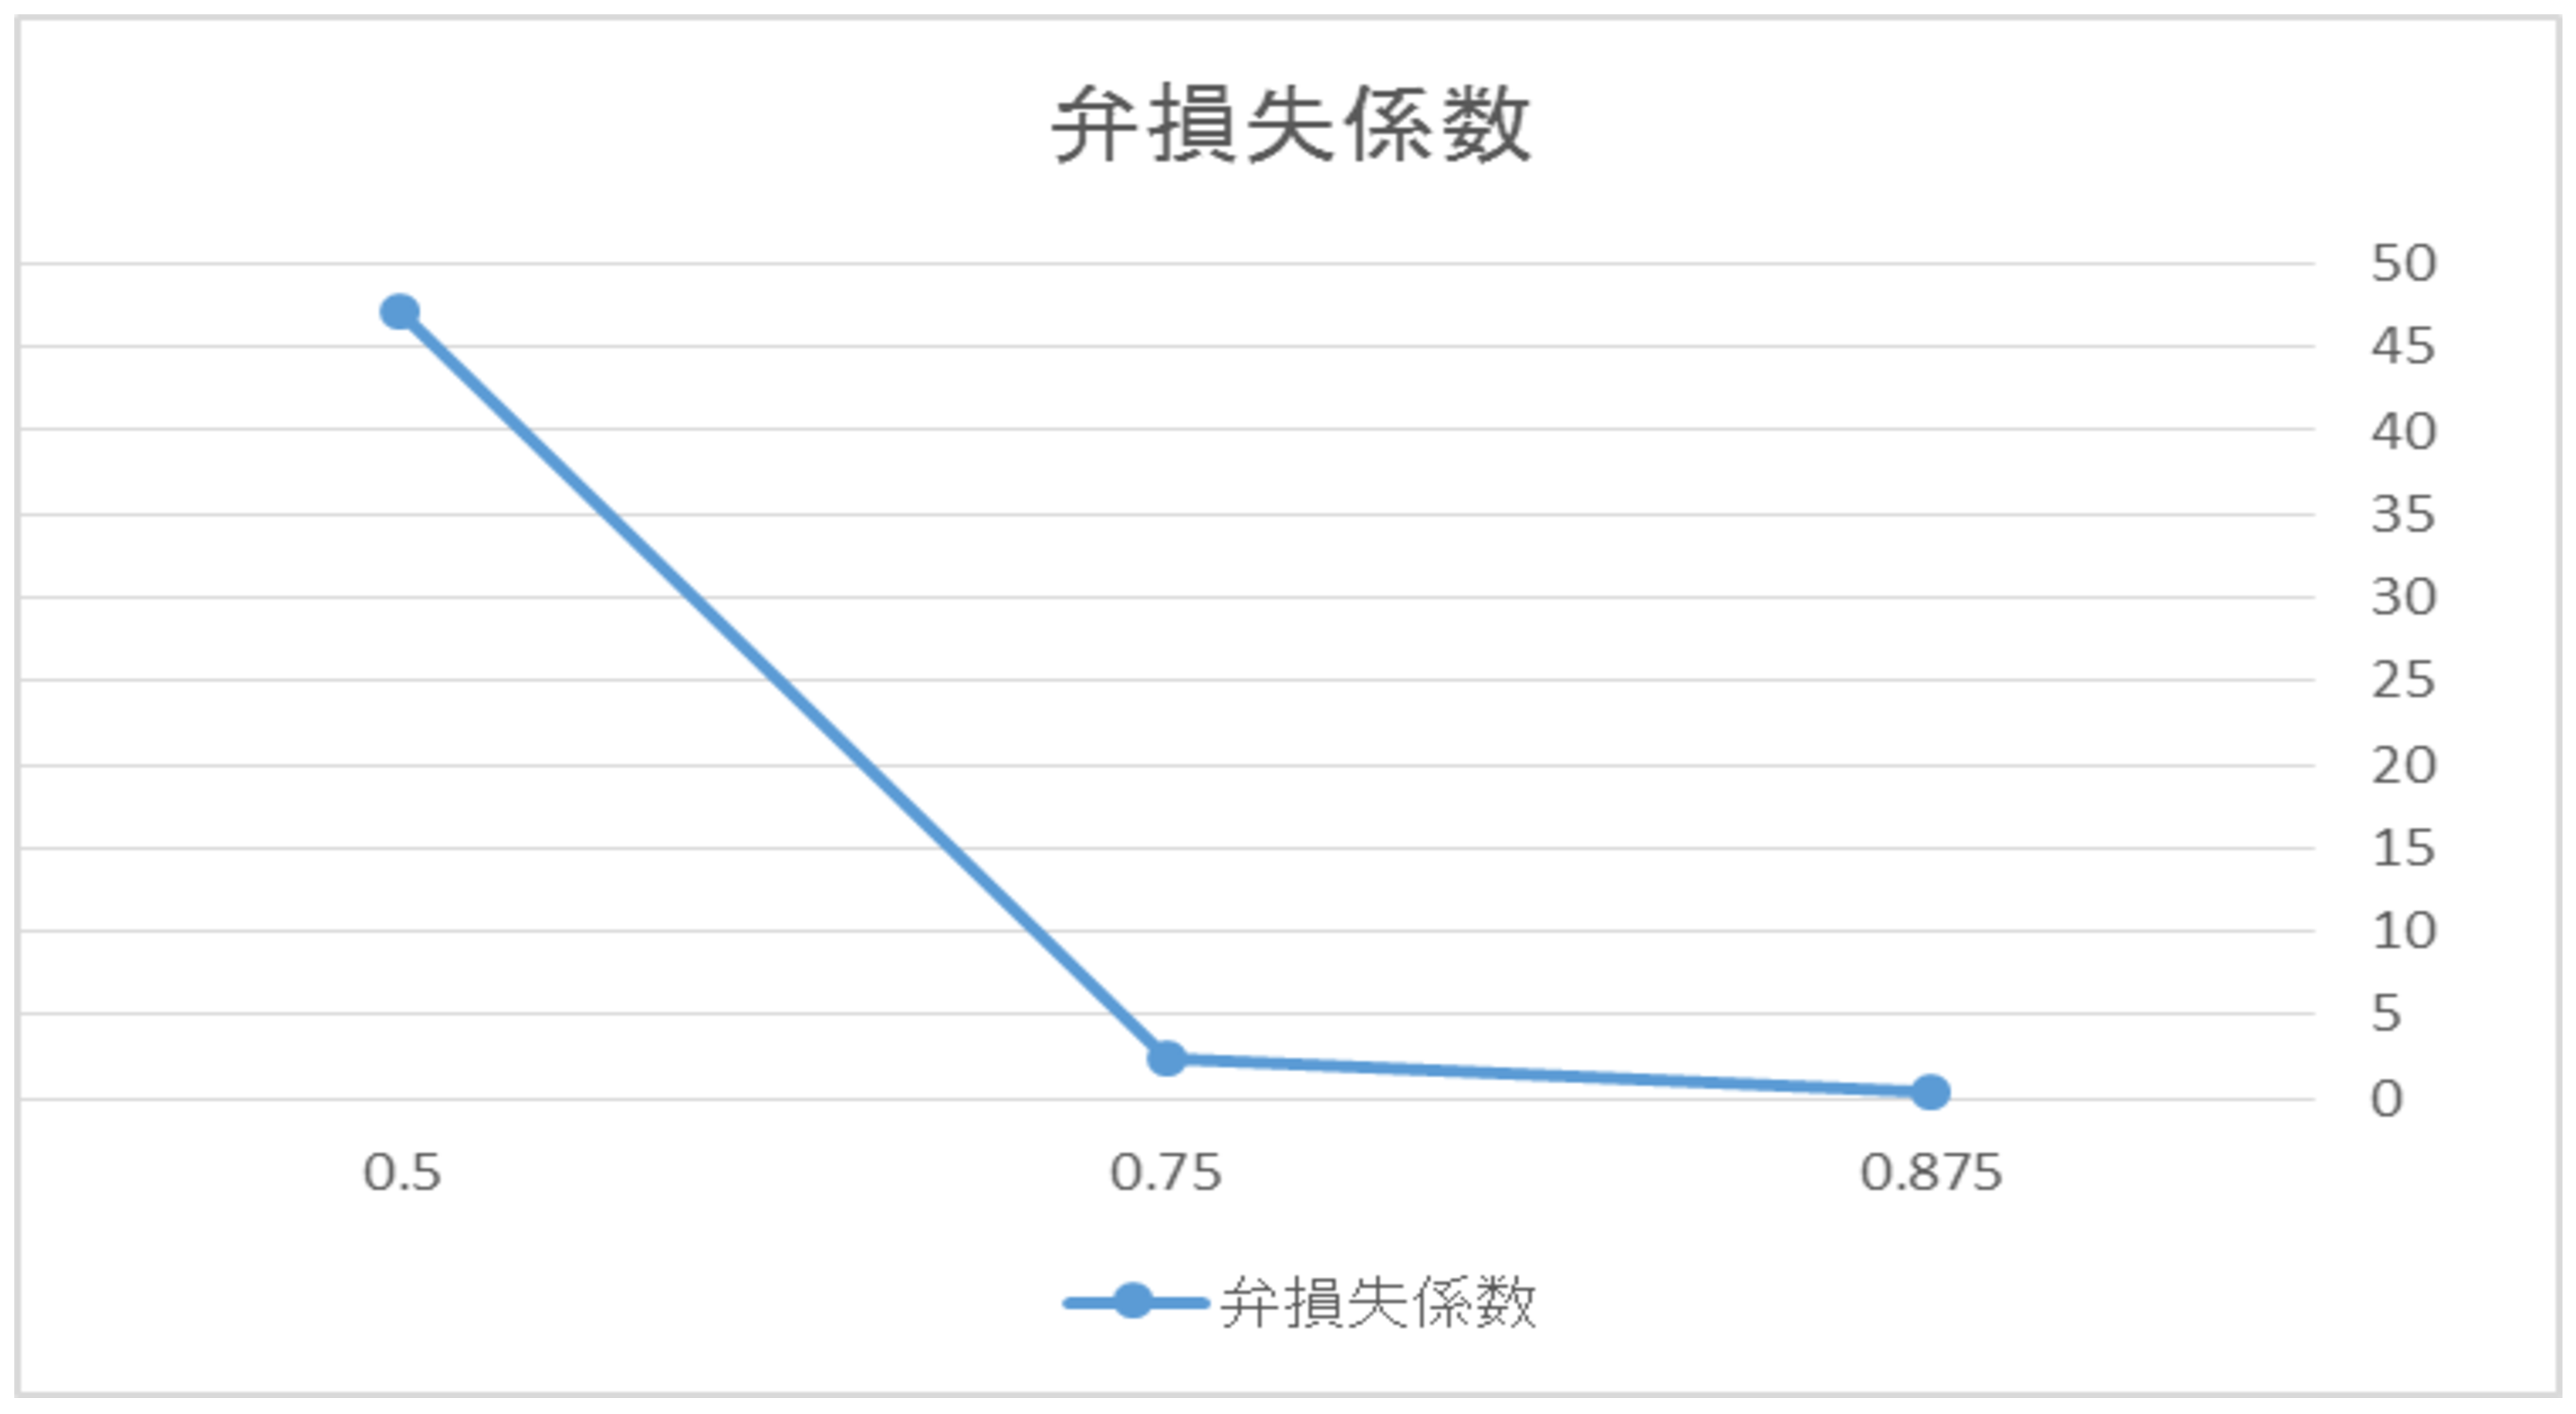
\includegraphics[width=12cm]{5.eps}
\end{center}
\caption{ボール弁開度と損失係数(横軸:ボール弁開度 縦軸:損失係数)}
\end{figure}
\newpage
\section{考察}
\begin{enumerate}
\item 実験結果の解釈
\begin{itemize}
\item HとVの予測精度\\
実験結果と予測値の正規化相互相関(NCC:Normalized Cross-Correlation)の値を求めると、0.9999579という結果が算出される。1に十分近い値が算出されたので,予測データと実験値の相関は非常に高いものと判断される。\\
\par
正規化相互相関の計算はYの値が$1300\sim500$の範囲とした。\\
ここで、xをサイフォンヘッドの値、予測した値をT(x),実験結果をI(x)とした。\\
\begin{equation}
NCC=\frac{\sum_{i=500}^{1300}T(i)I(i)}{\sqrt{\sum_{i=500}^{1300}T(i)^2+\sum_{i=500}^{1300}I(i)^2}}
\end{equation}
\item YとTの予測精度\\
下図に示すように一致していることがわかる。精度は整数値を保証している。


\item 無次元管内圧力Ps*から予測出来る事\\
この実験における無次元管内圧力の逆数は、出口のヘッド差によって与えられた(Ps-P0)の吸入圧力が、水にどのくらいエネルギを与えたかを示す指標(効率)となる数字である。今回の実験では、全開時に約1~12の値を示した。水位の低下によってこの効率は低下しているという事が分かる。また、弁を閉じるとこの効率は0に収束していく
\item 流量計としてエルボを使う事の妥当性\\
\begin{itemize}
\item エルボとベンド\\
エルボと同じ役割を担うものがベンドという管である。エルボの損失係数は1.0、対してベンドの損失係数は0.2~0.3であるが、ベンドは曲がるときの距離が長くなるので、どちらが良いかは使用条件で決定される。
\item エルボの圧力差と流量の関係\\
今回の実験により得られた流量係数とレイノルズ数のグラフを見ると、流量係数の値は、分散はあるが一定の値を取っている事が理解できる。流量係数の式は以下の通りである。

ここで実際にエルボ差圧を用いて流速を求めてみる。流量係数の平均値は27.2389であるので、
\end{itemize}




\item ボール弁損失係数の特徴
\end{itemize}
\item データ整理でエネルギー修正係数k=1と置いた取扱いの妥当性\\
エネルギー修正係数は次式で与えられる。
\begin{equation}
k=\int_0^{d/2}\frac{\rho u^2}{2}2 \pi rudr/(Q\frac{\rho V^2}{2})=\frac{8}{d^2V^3}\int_0^{d/2}u^3rdr
\end{equation}
この実験におけるレイノルズ数は、$R_e\geq 2300$であるので、次の式を用いて乱流における速度分布を推測する。
\begin{equation}
\frac{u}{U}=(1-\frac{y}{d/2})^{1/n}
\end{equation}
ここで、$n=3.45{R_e}^{0.07}$であるので、これを適用して
\begin{equation}
u=U (1-\frac{y}{d/2})^{1/(3.45{R_e})^{0.07}}
\end{equation}
参考文献1の7.12式により、
\begin{equation}
\frac{V}{U}=\frac{2n^2}{(n+1)(2n+1)}
\end{equation}
ここで、kの積分計算式を式変形すると、次のようになる。
\begin{eqnarray}
k&=&\frac{8}{d^2V^3}\int_0^{d/2}u^3rdr\nonumber\\
 &=&\frac{8}{d^2V^3}\int_0^{d/2}U^3 (1-\frac{y}{d/2})^{\frac{3}{n}}(\frac{2}{d}-y)(-dy)\nonumber\\
 &=&\frac{8}{d^2}(\frac{(n+1)(2n+1)}{2n^2})^3\int_0^{d/2}(1-\frac{y}{d/2})^{\frac{3}{n}}(\frac{2}{d}-y)(-dy)
\end{eqnarray}
ここで、$x=(1-\frac{y}{d/2})$とおくと、
\begin{eqnarray}
k&=&\frac{8}{d^2}(\frac{(n+1)(2n+1)}{2n^2})^3\int_1^{0}(x)^{\frac{3}{n}}\frac{d}{2}(1-x)(-\frac{d}{2}dx)\nonumber\\
 &=&\frac{8}{d^2}(\frac{(n+1)(2n+1)}{2n^2})^3\int_0^{1}\frac{d^2}{4}(x)^{\frac{3}{n}}(1-x)dx\nonumber\\
 &=&2\left(\frac{(n+1)(2n+1)}{2n^2}\right)^3\int_0^{1}(x)^{\frac{3}{n}}(1-x)dx\nonumber\\
 &=&2\left(\frac{(n+1)(2n+1)}{2n^2}\right)^3(\frac{n}{n+3}-\frac{n}{2n+3})\nonumber\\
 &=&\frac{(n+1)^3(2n+1)}{4(n+3)(2n+3)}
\end{eqnarray}
ここにnを代入する。今回の実験でのnの値は、約7.59$\sim$7.81程の値を取るので、代入するとkの値は、約1.05程の値を取る。\\
この実験において、管内の流れを非定常流れとしてエネルギー式をたてると、以下のようになる。
\begin{equation}
\int_A^C \frac{1}{g}\frac{\partial V}{\partial t}dx +\frac{P_c-P_A}{\rho g}+\frac{kV_C^2 - kV_A^2}{2g} + (Z_c - Z_A) +\Delta h = 0
\end{equation}
この式の中で、kの値が関係してくるのは第3項であるが、この項を実際に計算してみると、値としては約0.3というスケールである。対して$\Delta h$は、$0.4 \sim 1.2$、第4項の$(Z_C-Z_A)$は$1.48$から水位によって現象していく。このような関係性から、第3項のkの値が1.00であっても1.05であっても大きく影響することは無い。よって、k=1としたのは妥当である。
\item 実験中に水槽水面は低下するがHとVの関係を定常流として求めた妥当性
エネルギー式に境界条件を代入して整理すると、以下のようになる
\begin{equation}
\frac{dV_C}{dt}=\frac{g}{c}H-(1+\zeta_T)\frac{V_C^2}{2L}
\end{equation}
定常流として見るのであれば、上の式の値は0に近くならなければいけない。実際に値を代入した結果を以下に示す。
\begin{table}[htb]
\begin{center}
  \caption{$\frac{dV_C}{dt}$の算出結果}\tiny
  \begin{tabular}{|l||c|c|c|c|c|c|c|c|c|} \hline
サイホンヘッド&入口損失&管摩擦損失・垂直上昇&曲がり損失上流側エルボ&管摩擦損失水平菅&曲がり損失・下流側&管摩擦損失垂直下降&全損失&$\zeta_T$ & dVc/dt\\\hline
1.480&0.000&0.000&0.000&0.000&0.000&0.000&0.000&&\\
1.430&0.006&0.138&0.360&0.131&0.360&0.203&1.196&3.761&-0.192\\
1.380&0.006&0.136&0.355&0.130&0.355&0.200&1.183&3.763&-0.267\\
1.330&0.006&0.129&0.334&0.123&0.334&0.190&1.115&3.774&-0.183\\
1.280&0.006&0.125&0.321&0.119&0.321&0.183&1.074&3.782&-0.178\\
1.230&0.006&0.122&0.312&0.116&0.312&0.179&1.047&3.787&-0.213\\
1.180&0.005&0.116&0.295&0.110&0.295&0.170&0.992&3.797&-0.168\\
1.130&0.005&0.108&0.274&0.103&0.274&0.160&0.924&3.812&-0.083\\
1.080&0.005&0.104&0.261&0.099&0.261&0.153&0.883&3.821&-0.077\\
1.030&0.004&0.101&0.253&0.096&0.253&0.149&0.855&3.827&-0.111\\
0.980&0.004&0.098&0.244&0.093&0.244&0.144&0.828&3.834&-0.145\\
0.930&0.004&0.095&0.235&0.090&0.235&0.140&0.800&3.841&-0.178\\
0.880&0.004&0.089&0.218&0.085&0.218&0.131&0.745&3.856&-0.132\\
0.830&0.004&0.086&0.210&0.082&0.210&0.126&0.717&3.864&-0.165\\
0.780&0.003&0.080&0.193&0.076&0.193&0.117&0.661&3.881&-0.118\\
0.730&0.003&0.075&0.180&0.071&0.180&0.110&0.620&3.895&-0.111\\
0.680&0.003&0.072&0.171&0.068&0.171&0.106&0.592&3.904&-0.143\\
0.630&0.003&0.067&0.158&0.064&0.158&0.099&0.549&3.920&-0.135\\
0.605&0.002&0.057&0.133&0.055&0.133&0.085&0.465&3.957&0.052\\
0.580&0.002&0.041&0.090&0.039&0.090&0.060&0.321&4.041&0.407\\
0.555&0.000&0.007&0.013&0.007&0.013&0.011&0.051&4.525&1.119\\
0.552&0.000&&0.000&&0.000&&&&\\
\hline
  \end{tabular}
\end{center}
\end{table}
\normalsize
表より、弁を操作しないろきの実験結果は約$0.1\sim0.3$の値をとる。よって、これを0とすると、水深と経過時間の関係は連続の式で求められる。
\item 電磁流量計の動作原理
 電磁流量計はファラデーの電磁誘導の法則を利用して、導電性の液体の速度を測る測定具である。菅をまたぐようにコイルを設置して、コイルにより磁力Bを与える。菅には液体が速度Vで流れており、管の直径をDとすると、次の関係が成り立つ。
起電力Eは流速Vに比例するので、この関係から流速Vを求める事が出来る。
\item サイホン管の応用例、サイホンコーヒーとしての利用例
サイホンコーヒーは1840年頃から使用され始めました。利点として、味の濃さを自由に調整できること、味にブレがないこと、特有の雰囲気が出せる事が挙げられます。ドリップコーヒーと比べると、味が比較的濃く出る分、様々な銘柄の違いを強調する事が出来るので、人気のあるコーヒー抽出法の一つです。
下ボールに入れられた水を沸騰させると、下ボール内で水蒸気圧が上昇します。その結果、下ボール内の圧力が上昇して、水を上ボールに押し上げます。上ボールにはコーヒー豆を挽いたものを設置していますので、上がってきた熱湯によってそのまま抽出されます。加熱をやめると、圧力が下がるので、下ボールにコーヒーが流れ込みます。こうしてコーヒーが淹れられます。
\end{enumerate}
\section{結論}
ベルヌーイの式によって、今回のサイフォン管の流れは簡単に予測することが可能である。
\section{参考位文献}
\begin{itemize}
\item 松永他 流れ学-基礎と応用 朝倉書店 72頁
\end{itemize}
\end{document}